\documentclass{article}
\usepackage{geometry}
\usepackage{amsmath}
\usepackage{graphicx}
\usepackage{enumitem}
\usepackage{bm}
\usepackage{float}
% added this to stop hbadness warning
\hbadness = 5000000

\geometry
{
	headheight = 4ex,
	includehead,
	includefoot,
	paper = a4paper,
	inner = 2.5cm,
	outer = 2.5cm,
	bindingoffset = 0.5cm,
	top = 2cm,
	bottom = 1.5cm
}


\title{\Huge Problem Set 2} 
\vspace{1cm}
\author {\Large Chara Tsirka 03315, Prodromos Avramidis 03291}

\begin{document}

\maketitle
\begin{center}
\vspace{1cm}

\includegraphics[width=0.3\textwidth]{uthlogo.png}
\vspace{2cm}
\end{center}
\begin{center}
  \Huge Neurofuzzy Computing \vspace{1cm}

  \Large Fall Semester 2023-2024 \vspace{1cm}

  \Large Professor: Dimitrios Katsaros
\end{center}


%Problem 1
\newpage
\noindent \textbf{Problem 1}

\noindent Find the minimum of the two-dimensional function: $F(w) = w_1^2+w_2^2+(0.5w_1+w_2)^2+(0.5w_1+w_2)^4$
\\ 

\begin{figure}[h]
  \centering
  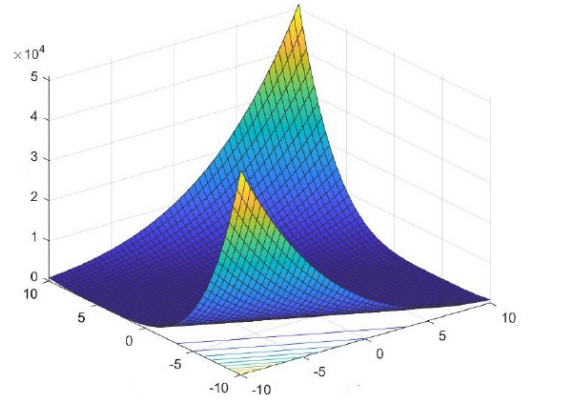
\includegraphics[width=0.4\textwidth]{pr1_a.png}
  
\end{figure}

\noindent with the Conjugate Gradient (Fletcher-Reeves), with initial guess $w(0)= [3, 3]^T$. Perform 
five iterations (if not finding the minimum earlier). Observe and comment on the 
slow/fast convergence towards the minimum $w=(0, 0)^T$. Then, apply the Gradient 
Descent method (accuracy: three decimal points) on the same function and unit step
movement. Perform ten iterations (if not finding the minimum earlier). For each method 
show your analytic calculations. \\ \\ \\


\noindent \underline{\textbf{\textit{Solution:}}}

%Problem 2
\newpage
\noindent \textbf{Problem 2}

\noindent Find the minimum of the previous function using the Newton method and fixed step $ \lambda_k = 1$ (even though this is not a quadratic form). \\

\noindent \underline{\textbf{\textit{Solution:}}} \\ 

\noindent The attached code converges after 9 iterations with the min point being (0,0) = 0.



%Problem 3
\newpage
\noindent \textbf{Problem 3}

\noindent For the neural network shown below

\begin{figure}[h]
  \centering
  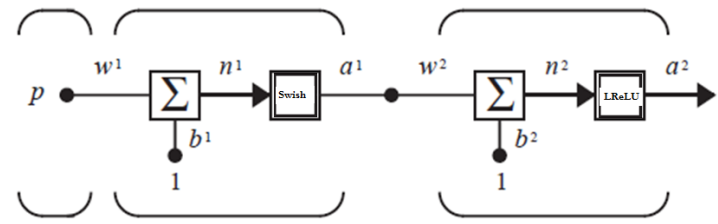
\includegraphics[width=0.4\textwidth]{pr3_a.png}
  
\end{figure}

\noindent the initial weights and biases are chosen to be $w^1(0) = -3, b^1(0) = 2, w^2(0) = -1, b^2(0) = -1$. An input/target pair is given to be ${\left \{p = 1, t=0 \right \} }$, and the parameter of LReLU is equal to 0.001. Perform two iterations of backpropagation with learning rate a=1.  \\ \\ \\


\noindent \underline{\textbf{\textit{Solution:}}}

\noindent The neural network shown above has two layers. The first layer's transfer function is Swish, so:
\[ F_1 = \frac{x}{1+e^{-x}}, (b=1) \]  
\[ F_1' = \frac{1+e^{-x} + xe^{-x}}{(1+e^{-x})^2}. \]
\\ \\The second layer's transfer function is LReLU with parameter equal to 0.001, so:
\[ F_2 = \begin{cases}
  0.001x & \text{for } x < 0 \\
  x & \text{for } x \geq 0 \\
\end{cases} \]
 
\[ F_2' = \begin{cases}
  0.001 & \text{for } x < 0 \\
  1 & \text{for } x \geq 0 \\
\end{cases}. \]\\

\noindent \textbf{\textit{First iteration of backpropagation:}}
\noindent \\ \\The output of the first layer is: \\ \\$n^1 = w^1p + b^1 = (-3)*1 + 2 \Rightarrow \bm{n^1 = -1}$
\\ \\$a^1 = F_1(n^1) = \frac{-1}{1+e} \Rightarrow \bm{a^1 \approx -0.2689}$

\noindent \\ \\The output of the second layer is: \\ \\$n^2 = w^2a^1 + b^2 = (-1)(-0.2689) + (-1) \Rightarrow \bm{n^2 \approx -0.731}$
\\ \\$a^2 = F_2(n^2) = 0.001(-0.731) \Rightarrow \bm{a^2 \approx -7.31 * 10^{-4}}$
\\ \\ \\The error is: \\$e = t - a^2 = 0 - (-7.31 * 10^{-4}) \Rightarrow \bm{e \approx 7.31 * 10^{-4}}$ 
\newpage 
\noindent We can now perform the backpropagation. The starting point is found at the second layer: \\ \\
$s^2 = -2F_2'(n^2)(t-a) = -2 * 0.001 * 7.31 * 10^{-4} \Rightarrow \bm{s^2 \approx -1.462 * 10^{-8}}$
\\\\ The first layer sensitivity is then computed by backpropagating the sensitivity from the second layer: \\ \\ $s^1 = F_1'(n^1)(w^2)^Ts^2 = \frac{1+e+(-1)e}{(1+e^x)^2} * (-1) *(-1.462 * 10^{-8}) \Rightarrow \bm{s^1 \approx 1.057 * 10^{-9}}$
\\\\ \\Finally, weight update takes place as follows: \\\\
$w^2(1) = w^2(0) - as^2(a^1)^T = -1 -1 * (-1.462 * 10 ^{-8}) * (-0.2689) \Rightarrow \bm{w^2(1) \approx -1.000000004}$
\\ \\ $b^2(1) = b^2(0) -as^2 = -1 -1 * (-1.462 * 10 ^ {-8}) \Rightarrow \bm{b^2(1) \approx 0.999}$
$\\ \\ \\ w^1(1) = w^1(0) -as^1(a^0)^T = -3 -1 * (1.057 * 10^{-9}) * $ 
\\ \\$b^1(1) = b^1(0) - as^1 = 2 - 1 * 1.057 * 10^{-9} \Rightarrow \bm{b^1(1) \approx 1.999}$\\ 

%Problem 4
\newpage
\noindent \textbf{Problem 4} \\

\noindent Write a (MATLAB/python/Keras/…) program to implement the backpropagation
algorithm for a $1-S^1-1$ network (logsig-ReLU). Write the program using matrix
operations, as we did in the class lecture. Choose the initial weights and biases to be
random numbers uniformly distributed between -0.5 and 0.5, and train the network to
approximate the function:
\begin{center}
  $ g(p)=1+sin[p(3 \pi /8)] for -2 \leq p \leq 2.$
\end{center}

\noindent Use $S^1=2, S^1=8, s^1=12$  Experiment with several different values for the learning
rate a (make sure you experiment with a = 0.1), and use several different initial conditions.
Discuss the convergence properties and the accuracy of the algorithm as the learning rate
changes, and as the capacity (in terms of number of hidden neurons) increases. \\ \\ \\

\noindent \underline{\textbf{\textit{Solution:}}} \\ 

\noindent We experimented with 3 different values for the learning rate a:
\begin{enumerate}
  \item For a = 0.01: \\
  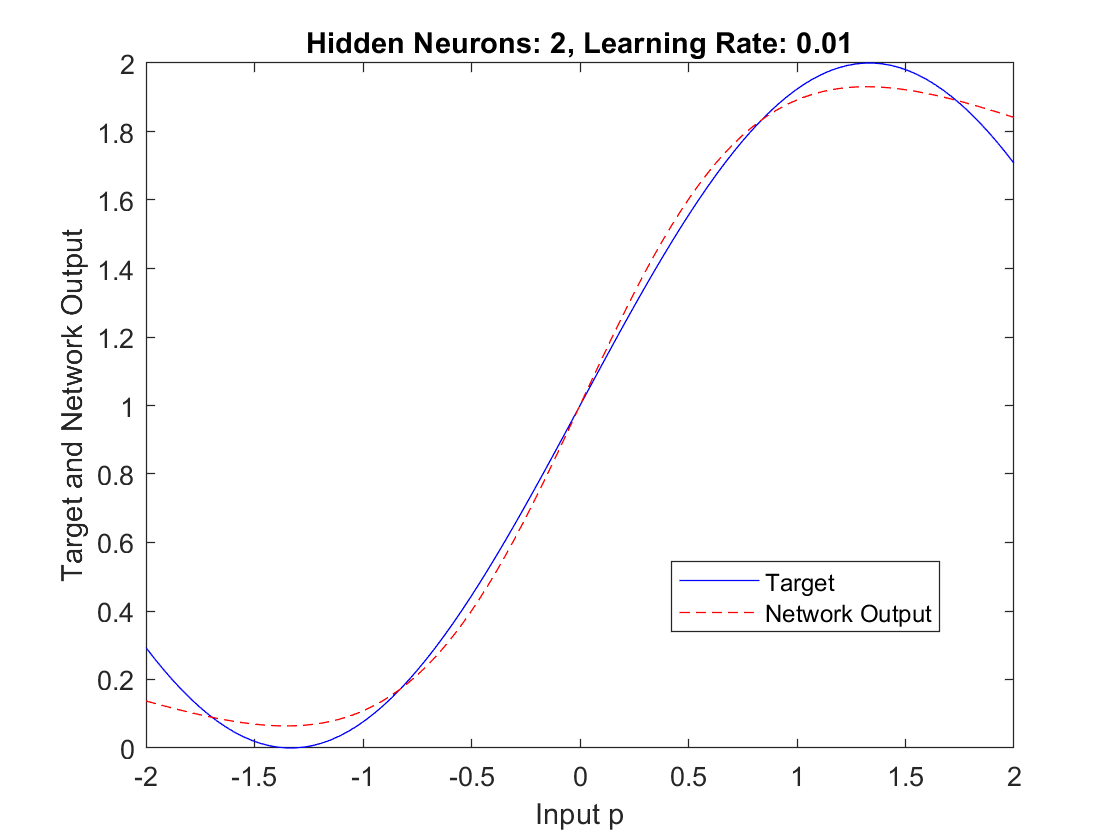
\includegraphics[width=0.3\textwidth]{Problem4_2_0.01.png}
  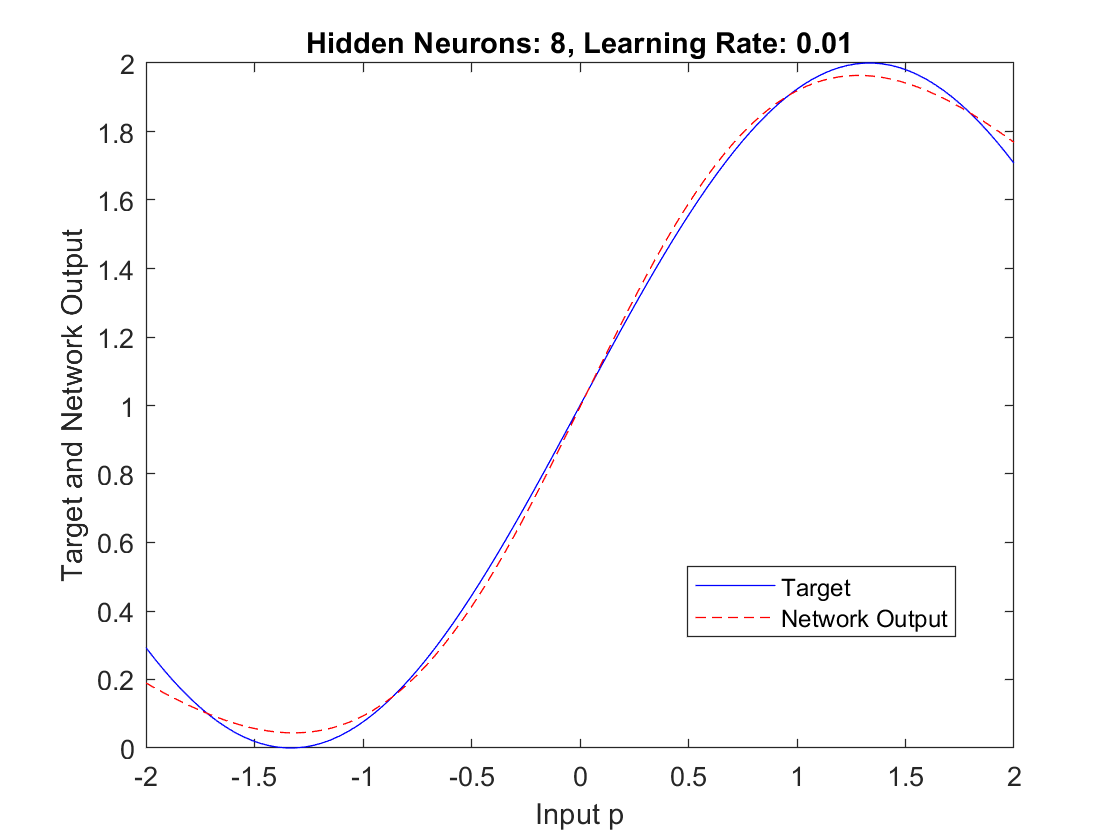
\includegraphics[width=0.3\textwidth]{Problem4_8_0.01.png}
  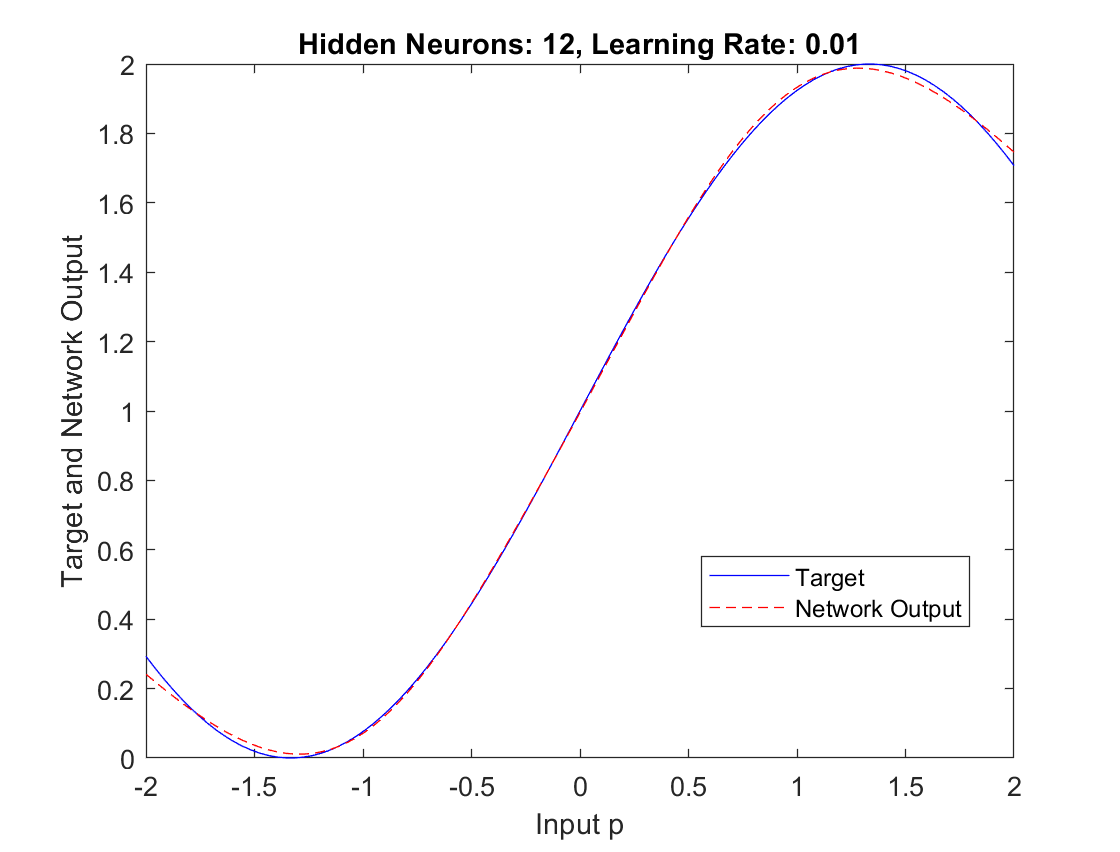
\includegraphics[width=0.3\textwidth]{Problem4_12_0.01.png}
  \item For a = 0.1: \\
  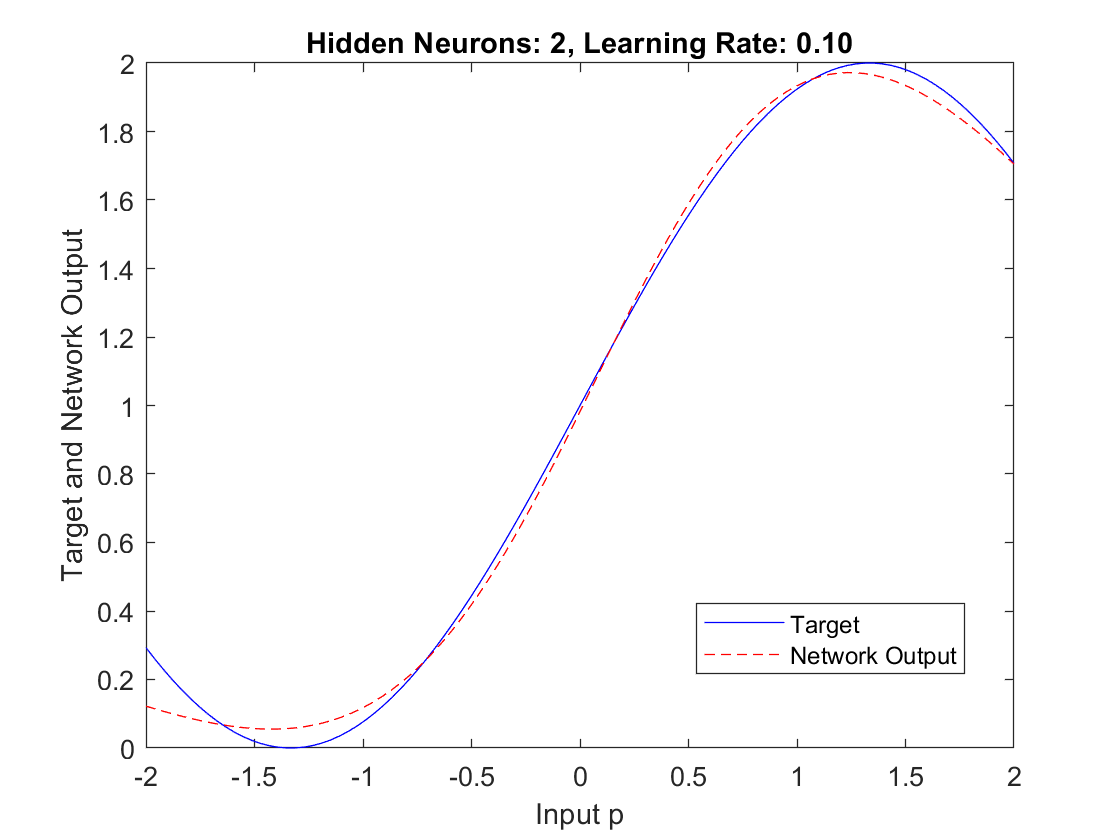
\includegraphics[width=0.3\textwidth]{Problem4_2_0.1.png}
  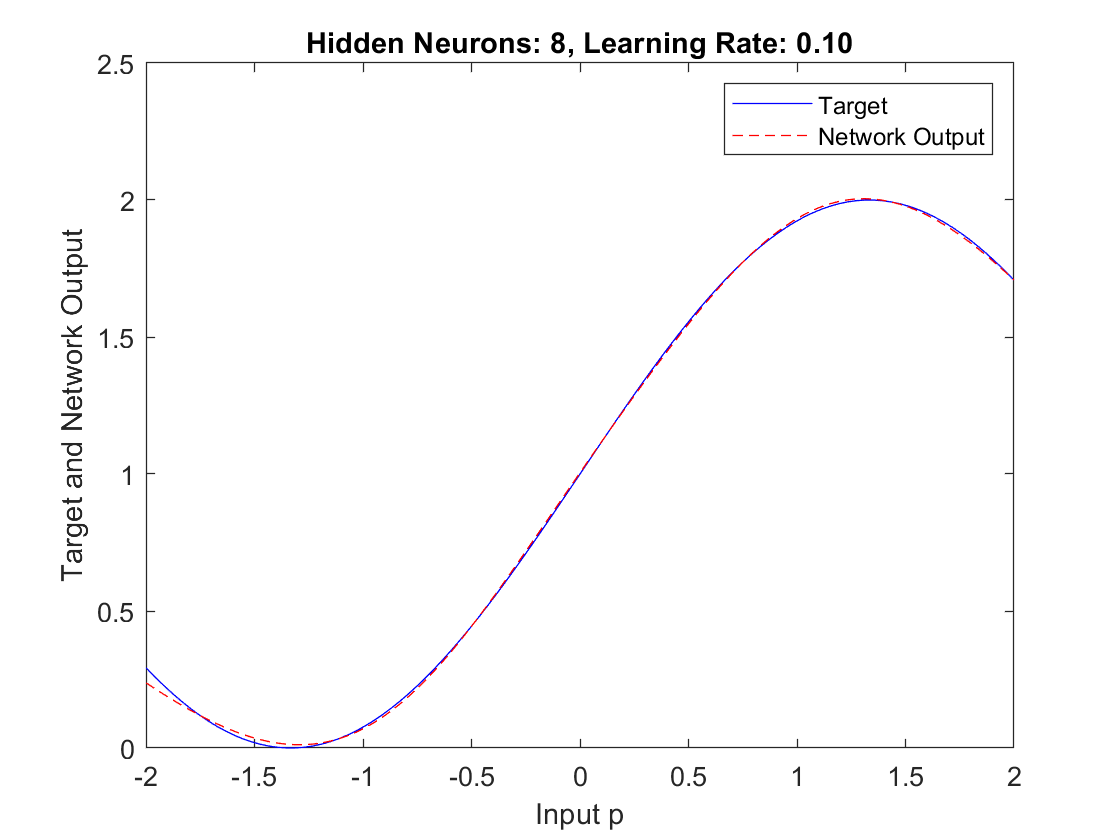
\includegraphics[width=0.3\textwidth]{Problem4_8_0.1.png}
  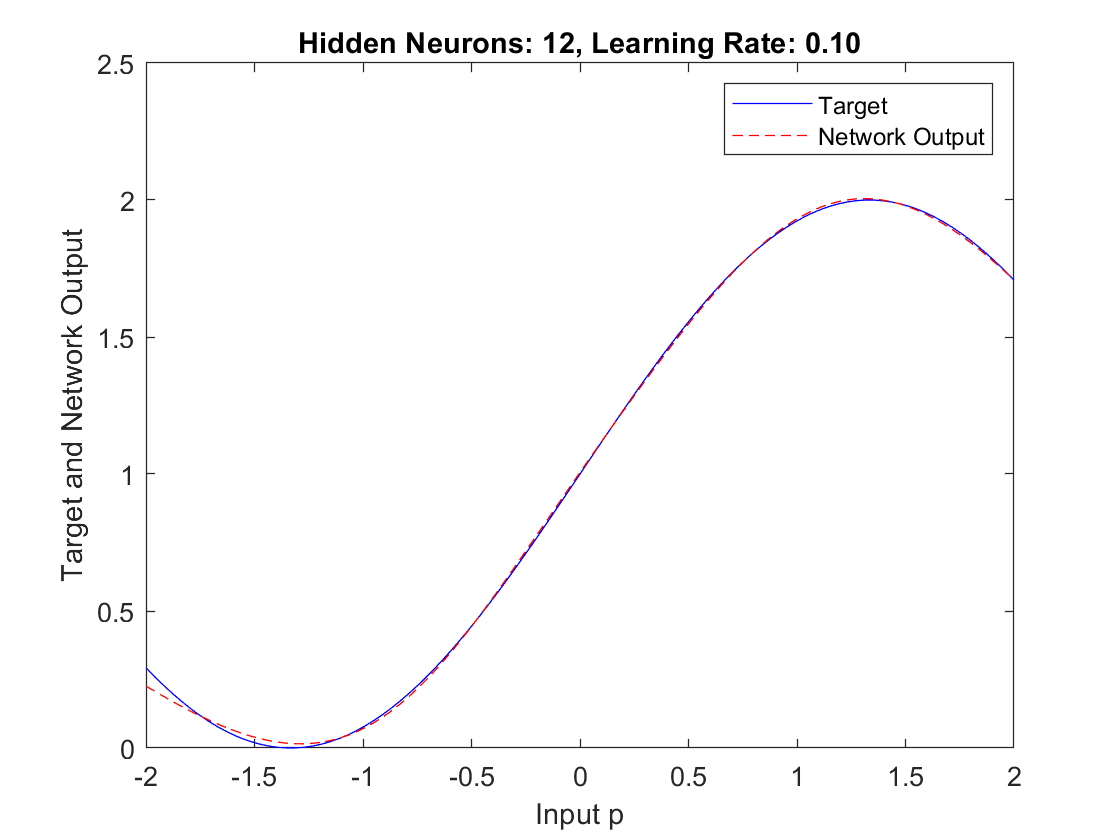
\includegraphics[width=0.3\textwidth]{Problem4_12_0.1.png}
  \item For a = 0.2: \\
  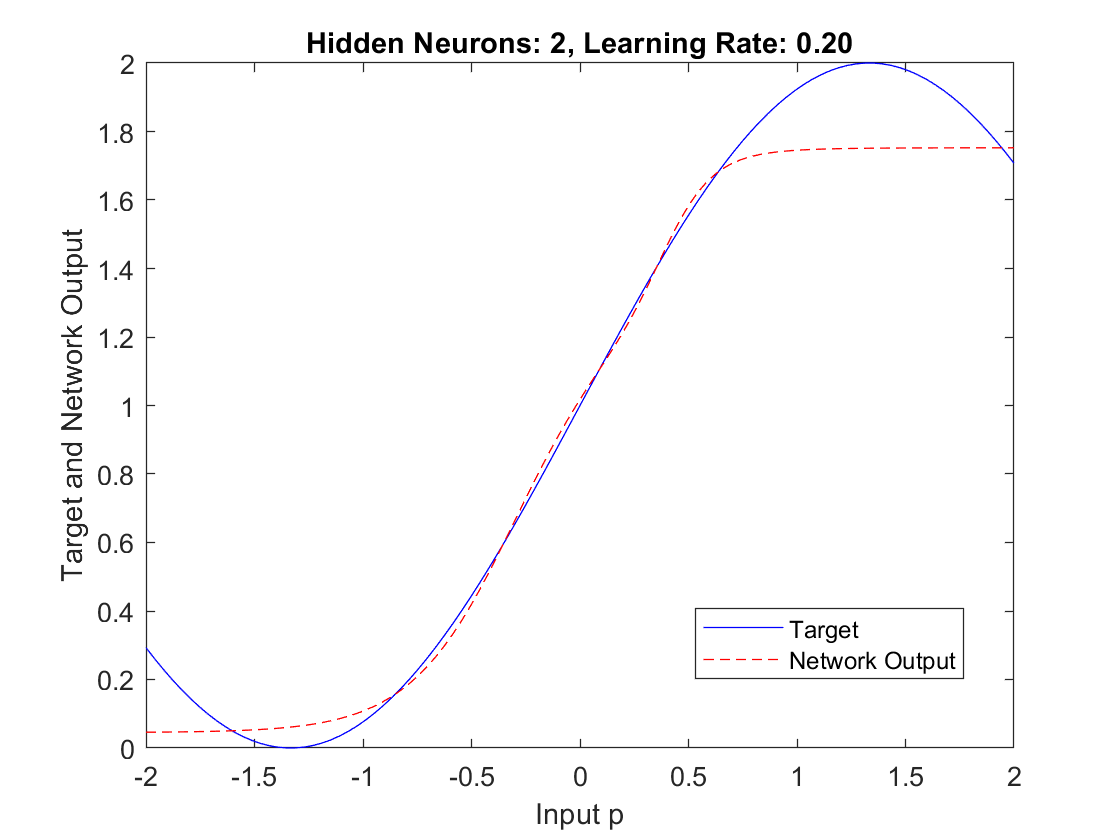
\includegraphics[width=0.3\textwidth]{Problem4_2_0.2.png}
  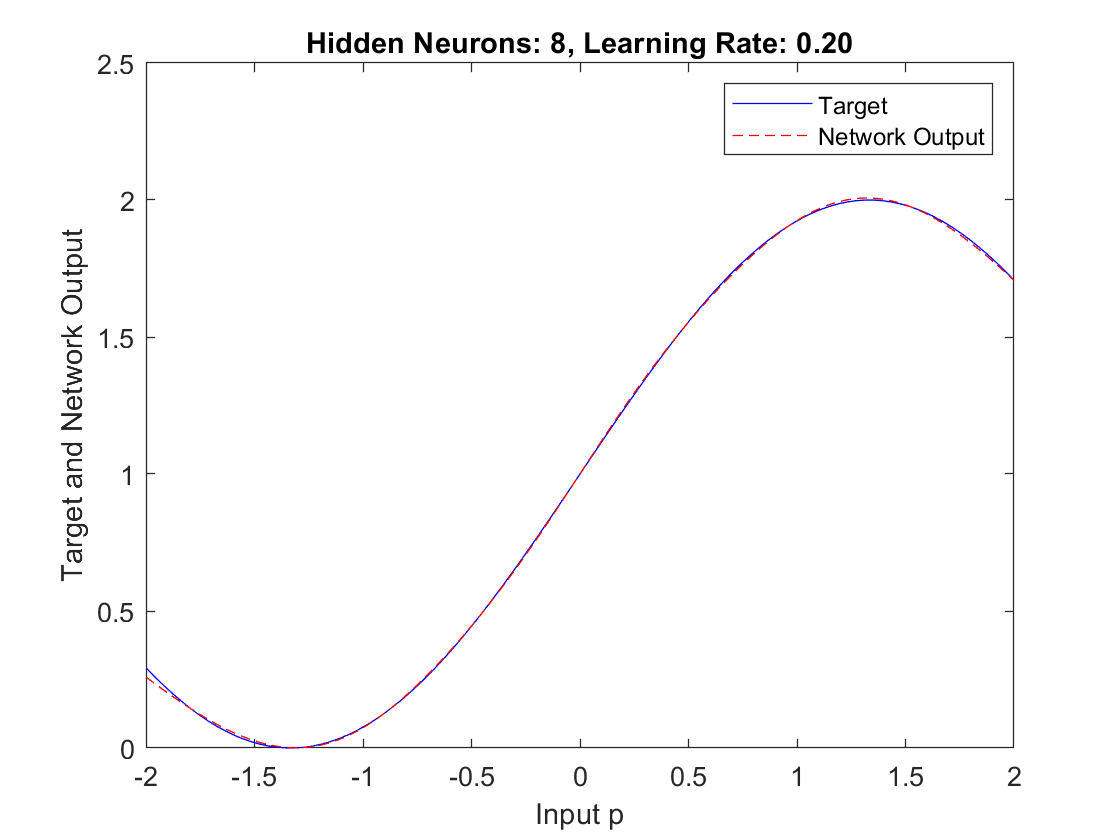
\includegraphics[width=0.3\textwidth]{Problem4_8_0.2.png}
  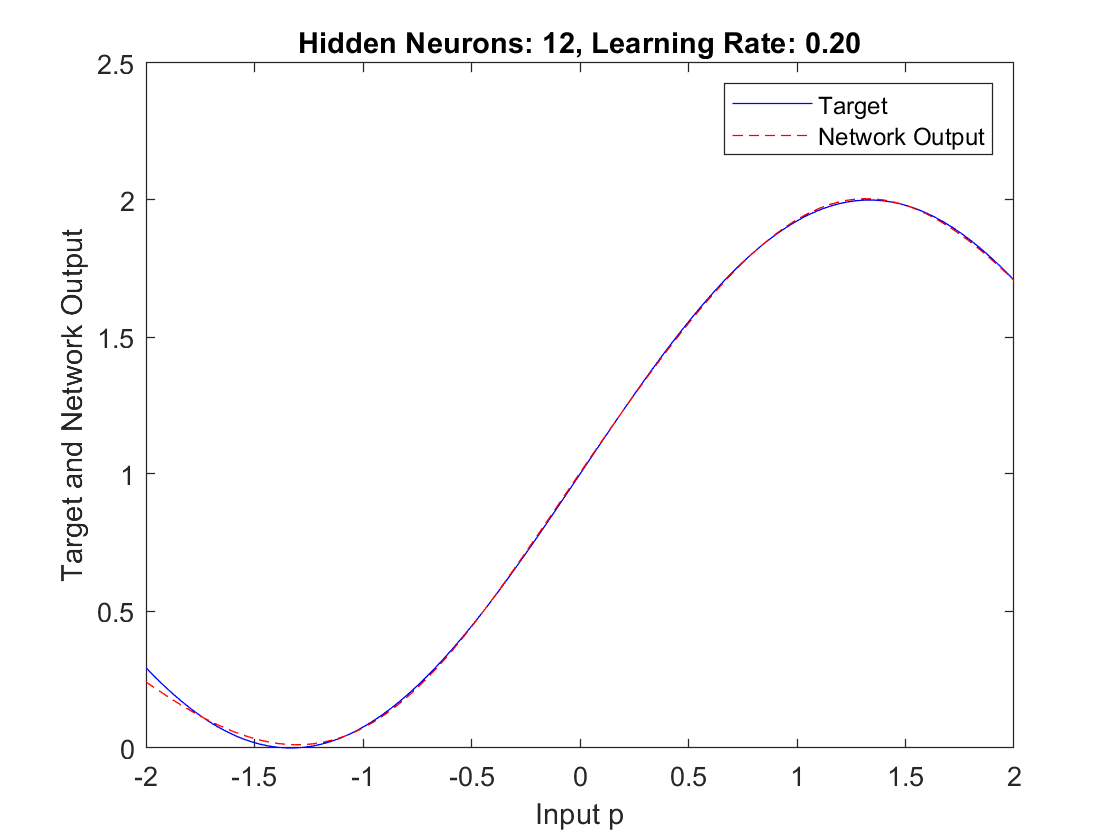
\includegraphics[width=0.3\textwidth]{Problem4_12_0.2.png}
\end{enumerate}

\noindent From the graphs we observe that:
\begin{enumerate}
  \item The more neurons a network has the more accurate it is.
  \item 
  As the number of neurons increases, the incremental improvement in accuracy becomes less noticeable, indicating diminishing returns.
  \item The graph becomes inaccurate when the learning rate is either too small or too large.
\end{enumerate}

%Problem 5
\newpage
\noindent \textbf{Problem 5} \\

\noindent In the setting with $S^1= 12$ and learning rate a=0.1 of the previous exercise, apply the
dropout technique (https://jmlr.org/papers/v15/srivastava14a.html) with dropout
probability $\theta$ of hidden-layer neurons equal to $\theta=0.15$, then with $\theta=0.25$, and then with
$\theta=0.35$. Apply the dropout during the training phase only, and only on the hidden layer
units (not of course to the input neuron). Discuss the convergence properties of the
algorithm, as well as its accuracy, and contrast your findings with those of the previous
exercise. Perform any additional experiments to figure out the operation of dropout as a
generalization technique. \\ \\ \\

\noindent \underline{\textbf{\textit{Solution:}}} 

\noindent For each of the $\theta$ values we get the following graphs:\\
\begin{enumerate}
  \item For $\theta=0.15:$ 
        \begin{figure}[h]
          \centering
          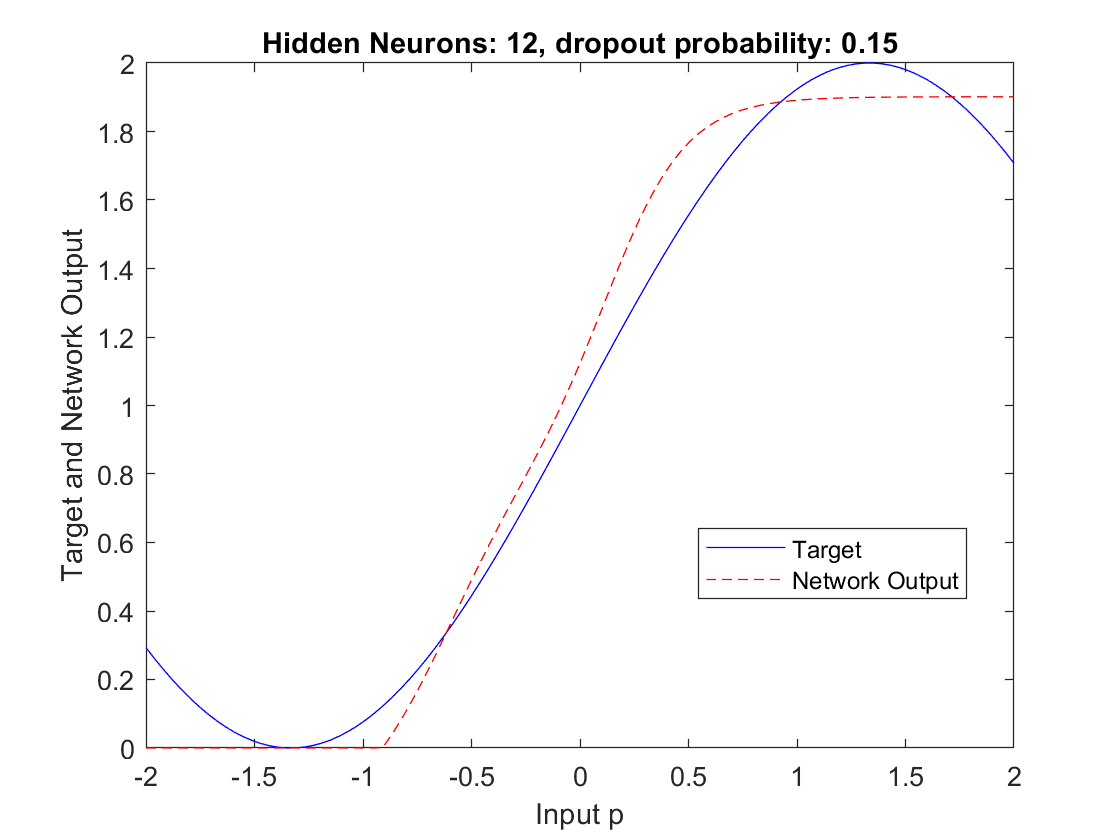
\includegraphics[width=0.5\textwidth]{Problem5_0.15.png}
        \end{figure}  
  \item For $\theta=0.25:$ 
        \begin{figure}[h]
          \centering
          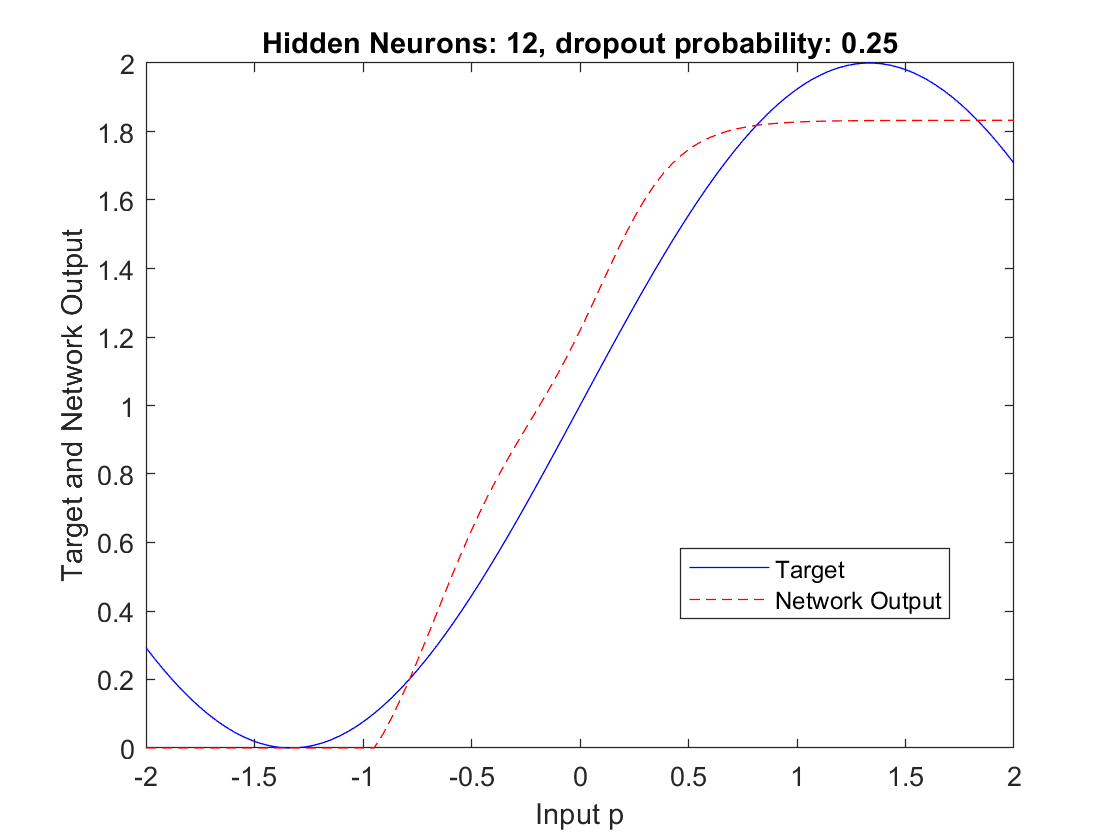
\includegraphics[width=0.5\textwidth]{Problem5_0.25.png}
        \end{figure} 
  \newpage
  \item For $\theta=0.35:$ 
        \begin{figure}[h]
          \centering
          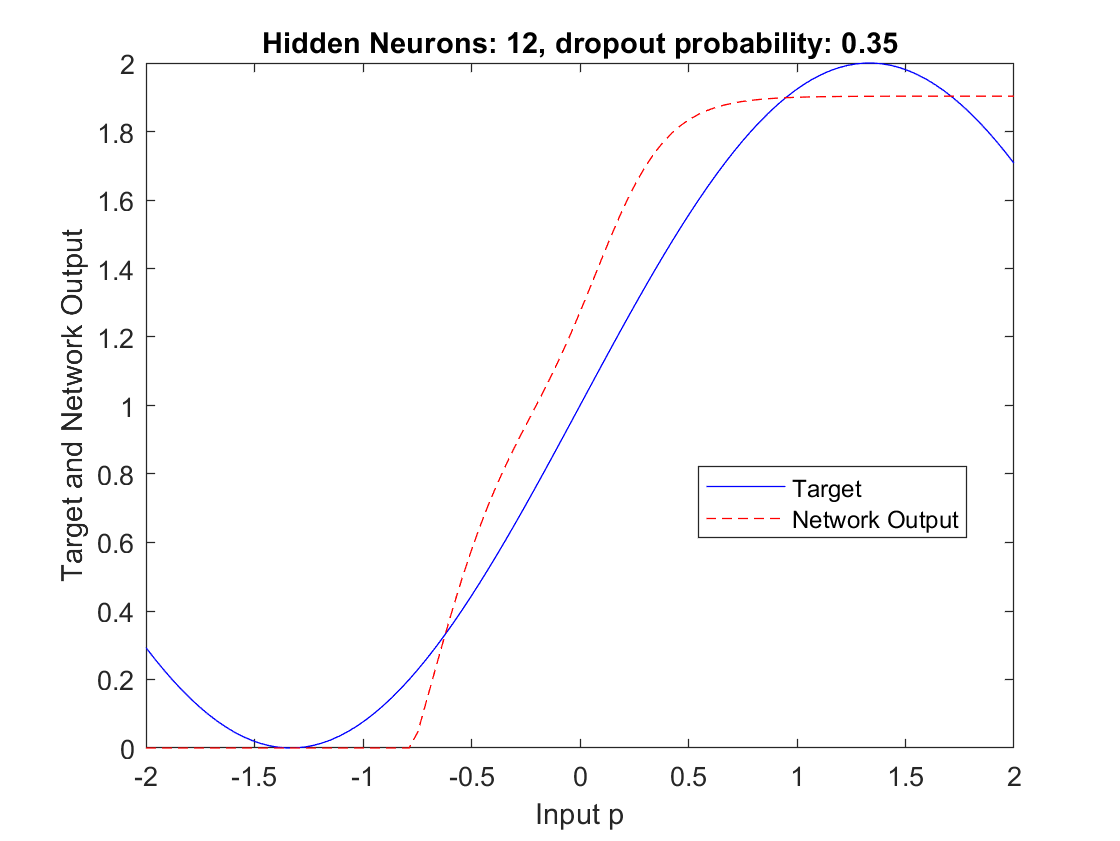
\includegraphics[width=0.5\textwidth]{Problem5_0.35.png}
        \end{figure}  
\end{enumerate} 
\noindent \\While the algorithm may not be as accurate as in Problem 4, we have successfully achieved our goal of preventing overfitting.




%Problem 7
\newpage
\noindent \textbf{Problem 7}

\noindent Show that an MLP using only ReLU (or pReLU) constructs a continuous piecewise linear function. \\ \\ \\

\noindent \underline{\textbf{\textit{Solution:}}}  

\noindent The ReLU function is defined as f(x) = max(0,x).\\
The pReLU function is defined as f(x) = max(ax,x) with a being a small coefficient.\\
In an MLP, each neuron computes a weighted sum of its inputs and applies an activation function to the sum. For a neuron 
with input x weight w and bias b the output before activation is w * x + b and after activation with ReLU it is max(0, w*x + b) while after pReLU it is max(a(w*x+b), w*x+b). \\

\noindent$\bm{Continuity:} $\\
Both the ReLU and pReLU functions are continuous functions. The MLP applies a continuous function for each layer so the overall function is also continuous.\\

\noindent$\bm{Piecewise}$ $ \bm{Linearity:} $\\
The ReLU function is piecewise linear, being linear (with a slope of 1) for positive inputs and zero elsewhere. \\
The pReLU function is also piecewise linear but with two linear pieces – one with a positive slope (usually 1) and another with a smaller positive slope (the parameter a). \\
In an MLP, each neuron applies a linear transformation (weighted sum) followed by a piecewise linear activation (ReLU/pReLU). This makes the output of each neuron piecewise linear. \\
The composition of piecewise linear functions remains piecewise linear. Thus, the entire network, being a composition of linear transformations and piecewise linear activations, represents a piecewise linear function.

\noindent In conclusion an MLP using only ReLU or pReLU constructs a continuous piecewise linear function.


%Problem 8
\newpage
\noindent \textbf{Problem 8} \\
Consider the following function:
\begin{center}
    $ F(w) = 0.1w_1^2 + 2w_2^2$
\end{center}

\begin{enumerate}
    \item Find the minimum of the function implementing the Adadelta optimizer (instead of
            gradient descent) with learning rate $\alpha = 0.4$. Plot the algorithm’s trajectory on a contour
            plot of F(x)
    \item Change the learning rate to $\alpha = 3$, and repeat the same task.
    \item Try out Adadelta for the same objective function rotated by 45degrees, i.e., 
            $ F(w) = 0.1(w_1+w_2)^2 + 2(w_1-w_2)^2$. Does it behave differently?\\ 
\end{enumerate} 

\noindent \underline{\textbf{\textit{Solution:}}} 

\begin{enumerate}
    \item For a = 0.4:
          \begin{figure}[h]
            \centering
            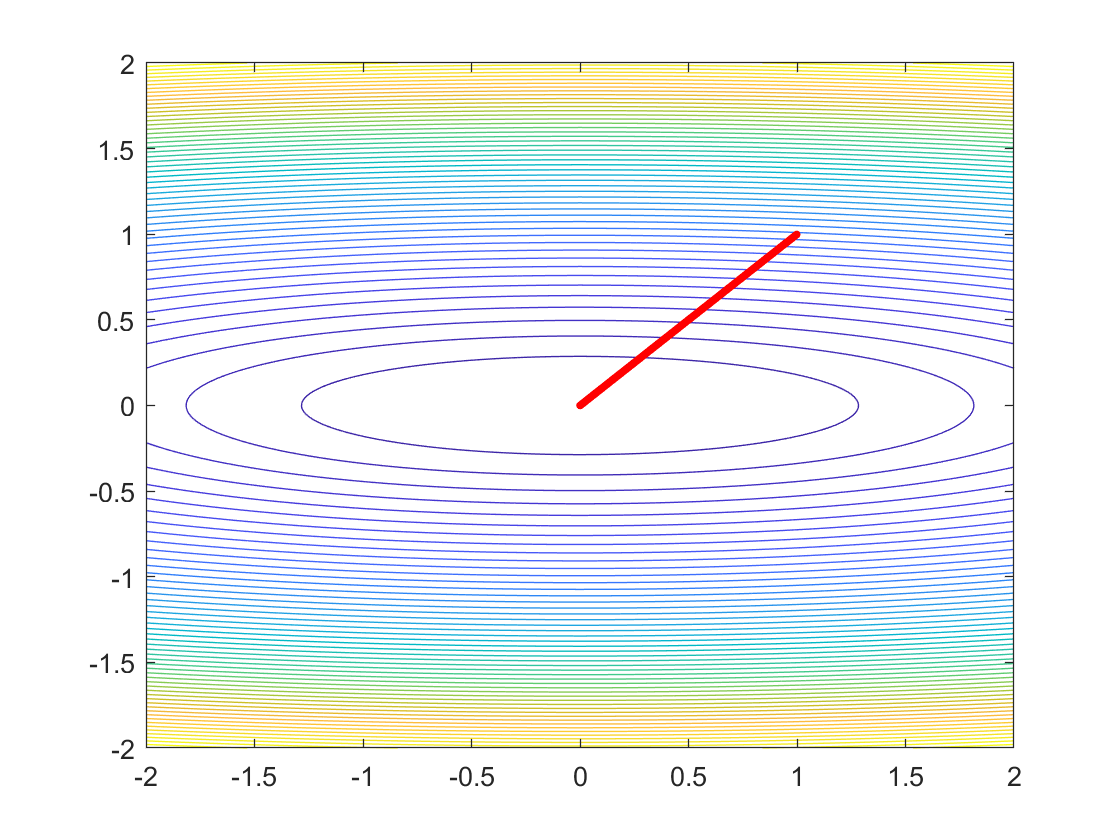
\includegraphics[width=0.5\textwidth]{problem80.4.png}      
          \end{figure}
    \item For a = 3:
          \begin{figure}[h]
            \centering
            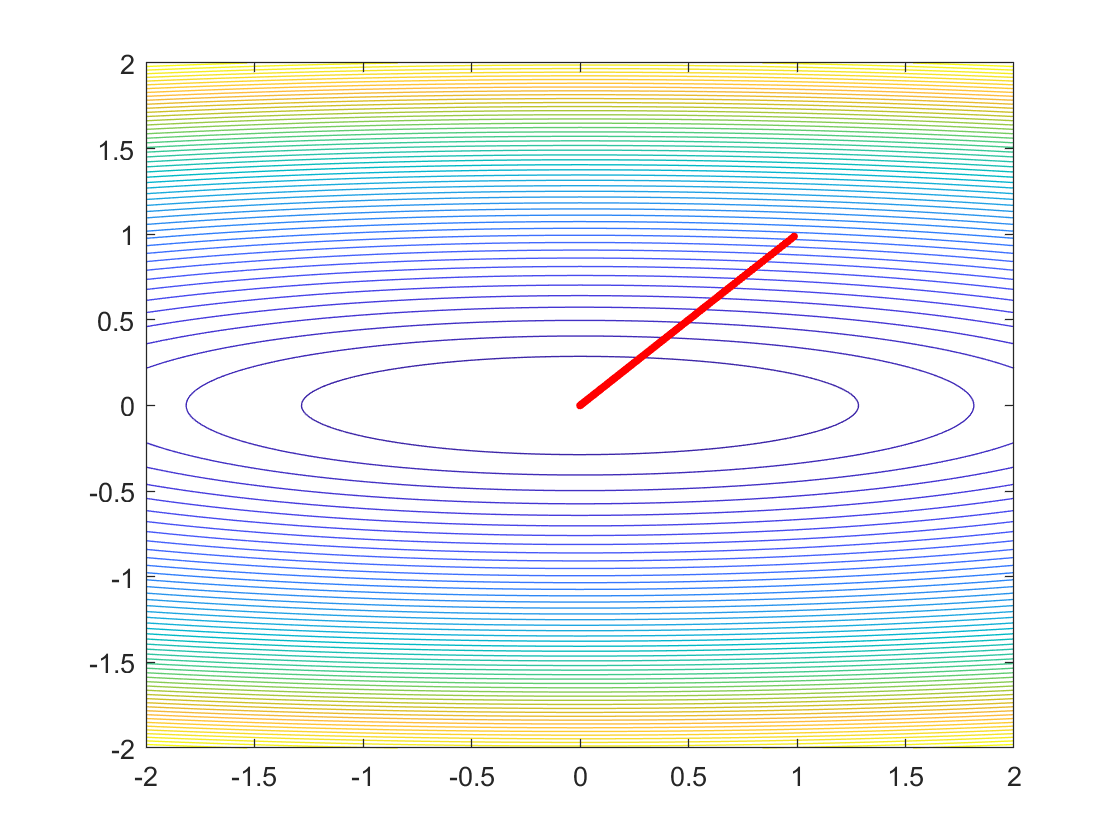
\includegraphics[width=0.5\textwidth]{problem83.png}            
          \end{figure} 
          \newpage
    \item Adadelta, fucntion rotated by 45 degrees:
          \begin{figure}[h]
            \centering
            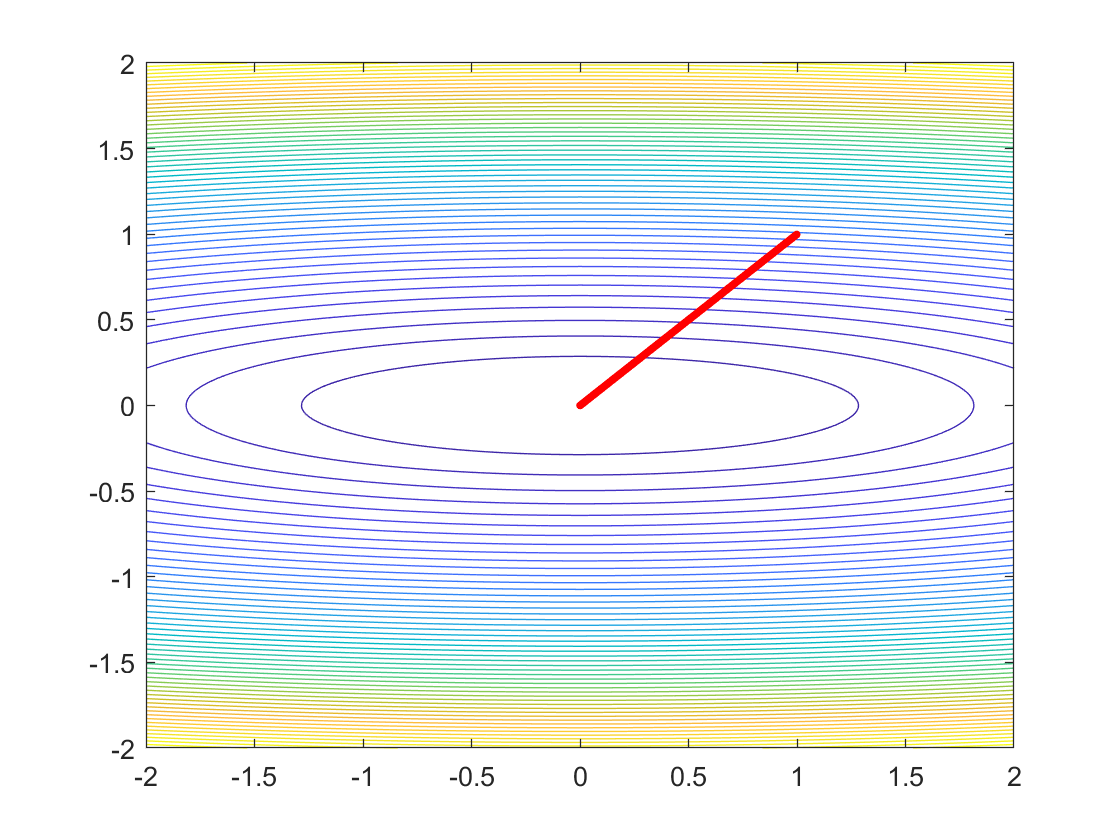
\includegraphics[width=0.5\textwidth]{problem8rotated.png}            
          \end{figure} 
          \noindent \\It does not behave differently. 
            
\end{enumerate}



%Problem 9
\newpage
\noindent \textbf{Problem 9} \\

\noindent On the plot below, show one gradient step (with an arrow) for each of the methods
mentioned below. The minimum is the black circle, whereas your position is the black 
square. Make sure you label the three arrows in your answer. 
\begin{enumerate}
  \item Standard gradient
  \item Natural gradient (or Newton’s method)
  \item Adagrad or RMSprop (assume they have run for a while to accumulate gradient
  information)
\end{enumerate}

\noindent Explain the direction of the arrow you designed. \\ \\

\noindent \underline{\textbf{\textit{Solution:}}} \\ 

\begin{enumerate}
  \item The plot after one gradient step for the Standard gradient method:
        \begin{figure}[h]
          \centering
          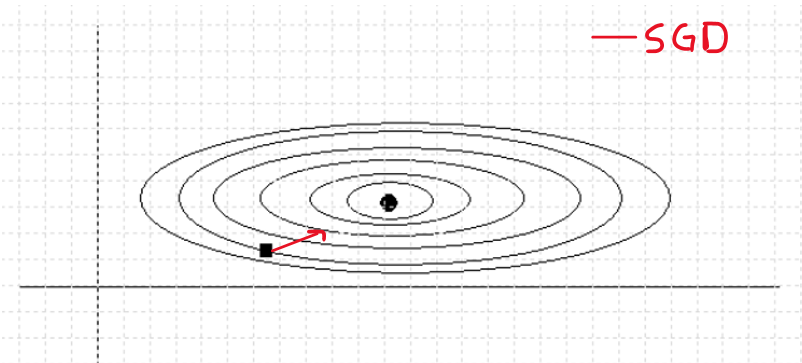
\includegraphics[width=0.6\textwidth]{pr9_a.png}
          
        \end{figure}
        
  \item The plot after one gradient step for the Natural gradient method:
        \begin{figure}[h]
          \centering
          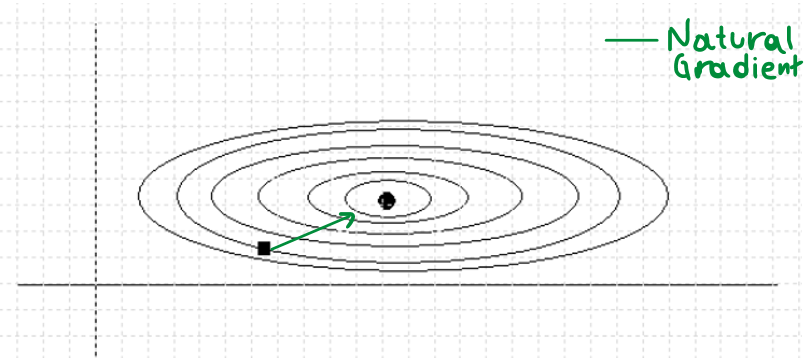
\includegraphics[width=0.6\textwidth]{pr9_b.png}
          
        \end{figure}
  \item The plot after one gradient step for the Adagrad or RMSprop method:
        \begin{figure}[h]
          \centering
          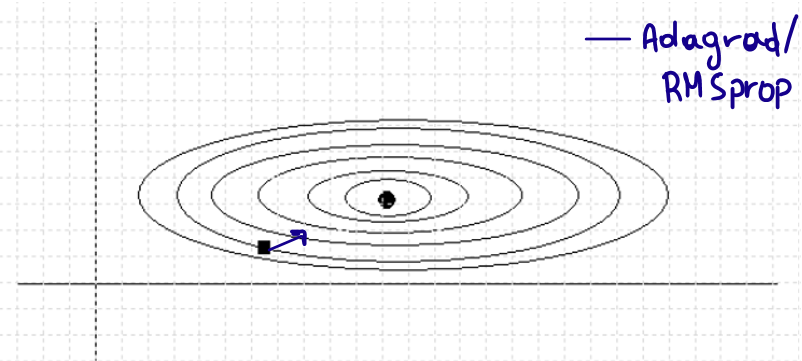
\includegraphics[width=0.6\textwidth]{pr9_c.png}
          
        \end{figure}
\end{enumerate}




%Problem 10
\newpage
\noindent \textbf{Problem 10} \\

\noindent You are given the description of the following optimization method, where $ \alpha, \beta, \nu \in R, (\alpha $
is the learning rate):

\begin{center}
$g_{t+1} \leftarrow \beta \cdot g_t + (1 - \beta) \cdot \nabla L_t(\theta_t) $
\end{center}
\begin{center}
$\theta_{t+1} \leftarrow \theta_t - \alpha \left[ (1 - \nu) \cdot \nabla L_t(\theta_t) + \nu \cdot g_{t+1} \right] $
\end{center}

\noindent For which values of $ \beta $ and $\nu$ you get optimization methods familiar to you (described in
our lectures)? Name them, and write the respective equations.\\ \\ \\

\noindent \underline{\textbf{\textit{Solution:}}}

\noindent The above equations can represent 3 different optimization methods:

\begin{enumerate}
  \item For $\beta = 0$ and $\nu = 0$  we get the standard gradient descent optimization method
    \begin{center}
    $g_{t+1} \leftarrow \nabla L_t(\theta_t) $
    \end{center}
    \begin{center}
    $\theta_{t+1} \leftarrow \theta_t - \alpha \cdot \nabla L_t(\theta_t)$
    \end{center}
    
  \item For $\beta \neq 0$ and $\nu = 0$ we get the SGD with monmentum optimization method
    \begin{center}
    $g_{t+1} \leftarrow \beta \cdot g_t + (1 - \beta) \cdot \nabla L_t(\theta_t) $
    \end{center}
    \begin{center}
      $\theta_{t+1} \leftarrow \theta_t - \alpha \cdot \nabla L_t(\theta_t)$
    \end{center}
    
  \item For $\beta \neq 0$ and $\nu \neq 0$ we get the Nesterov Accelerated Gradient optimization method
  \begin{center}
    $g_{t+1} \leftarrow \beta \cdot g_t + (1 - \beta) \cdot \nabla L_t(\theta_t) $
    \end{center}
    \begin{center}
    $\theta_{t+1} \leftarrow \theta_t - \alpha \cdot \nu \cdot g_{t+1} $
    \end{center}
\end{enumerate}







%Problem 11
\newpage
\noindent \textbf{Problem 11}

\noindent Consider the following input image: \\ \\
\begin{center}  

 $ I = \begin{bmatrix}
    20 & 35 & 35 & 35 &35 & 20 \\
    29 & 46 & 44 & 42 &42 & 27 \\
    16 & 25 & 21 & 19 &19 & 12 \\
    66 & 120 & 116 & 154 &114 & 62 \\
    74 & 216 & 174 & 252 &172 & 112 \\
    70 & 210 & 170 & 250 &170 & 110
  \end{bmatrix}$ 
\end{center}

\vspace{0.5cm}
\begin{enumerate} [label=\Alph*]
    
    \item  What is the output provided by a convolution layer with the following properties: \\ \\
        stride=(1, 1), and kernel = $\begin{bmatrix}
    1 & 1 & 1 \\
    1 & 0 & 1  \\
    1 & 1 & 1 \\
    
    \end{bmatrix}$
    \item Take the output from A. and apply a max pooling layer with the following properties: \\ \\
        stride=(2,2), window shape=(2, 2).
    \item For the following kernels, describe what kind of feature they extract from the image:
    \begin{center}  
         $ F1 = \begin{bmatrix}
            -10 & -10 & -10 \\
            5 & 5 & 5  \\
            -10 & -10 & -10 \\
          \end{bmatrix}$ 
\end{center}
\begin{center}  
         $ F2 = \begin{bmatrix}
            2 & 2 & 2 \\
            2 & -12 & 2  \\
            2 & 2 & 2 \\
          \end{bmatrix}$ 
\end{center}
\begin{center}
    $ F3 = \begin{bmatrix}
        -20 & -10 & 0 & 5 &10 \\
        -10 & 0 & 5 & 10 &5 \\
        0 & 5 & 10 & 5 &0 \\
        5 & 10 & 5 & 0 &-10 \\
        10 & 5 & 0 & -10 &-20 \\
    \end{bmatrix}$ 
\end{center}

    
\end{enumerate}

\noindent \underline{\textbf{\textit{Solution:}}} \\ 

\begin{enumerate} [label=\Alph*]
    \item The output is:
        \begin{center}
        $ I = \begin{bmatrix}
            225 & 258 & 250 & 209 \\
            458 & 566 & 552 & 372 \\
            708 & 981 & 887 & 802 \\
            1000 & 1488 & 1320 & 1224 
        \end{bmatrix}$ 
        \end{center}

    \item After the max pooling layer: 
        \begin{center}
        $ I = \begin{bmatrix}
            566 & 552 \\
            1488 & 1320
        \end{bmatrix}$ 
        \end{center}

    \item The image after each of the kernels: \\
        \begin{center}
            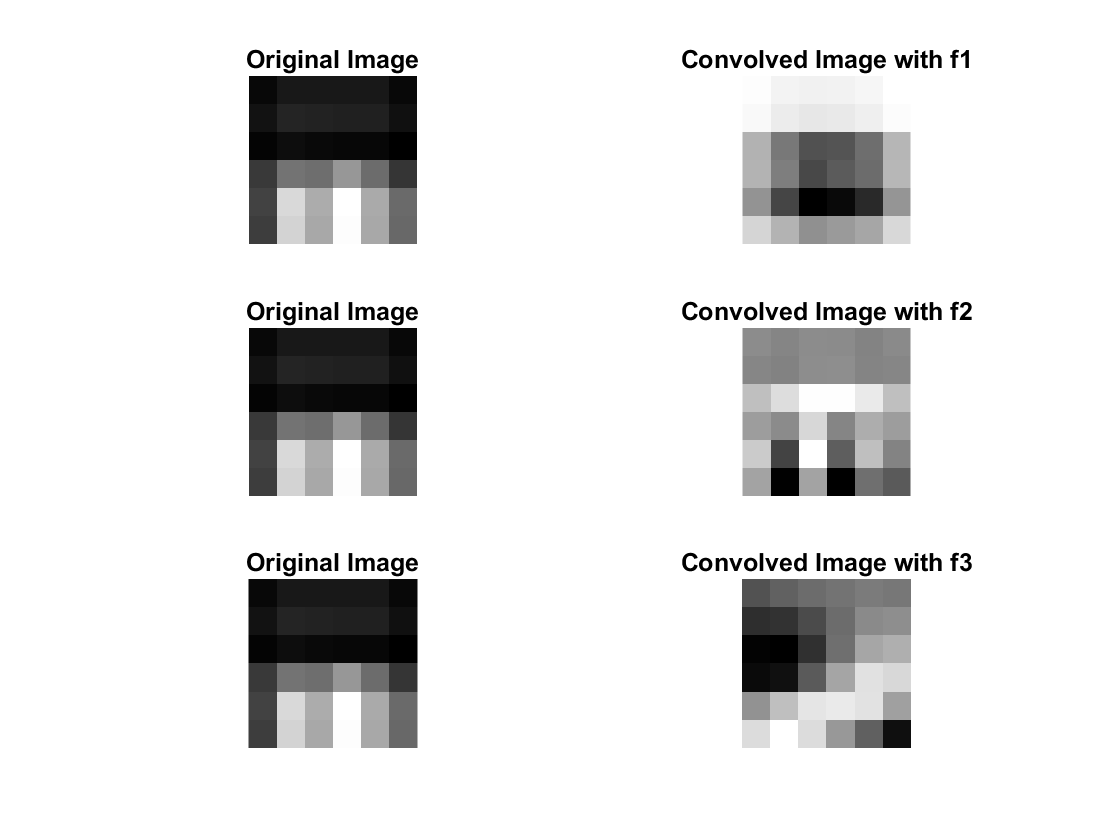
\includegraphics[width=0.4\textwidth]{problem11images.png}
        \end{center}
        F1 appears to detect horizontal edges , F2 detects edges in all directions and F3 detects edges on a diagonal.
        
            
\end{enumerate}\



%Problem 12
\newpage
\noindent \textbf{Problem 12}

\noindent Consider a 1D convolutional network where the input has three channels. The first 
hidden layer is computed using a kernel size of three and has four channels. The second
hidden layer is computed using a kernel size of five and has ten channels. How many 
biases and how many weights are needed for each of these two convolutional layers? \\ \\ \\

\noindent \underline{\textbf{\textit{Solution:}}} \\ 

\noindent \textit{First convolution layer:} \\ \\




%Problem 13
\newpage
\noindent \textbf{Problem 13}

\noindent Max-pooling can be accomplished using ReLU operations.
\begin{enumerate} [label=\Alph*]
    
    \item Express max(a, b) by using only ReLU operations.
    \item Use this to implement max-pooling by means of convolutions and ReLU layers.
    \item How many channels and layers do you need for a 2x2 convolution? How many for a 3x3 convolution?\\ \\ \\
\end{enumerate}\

\noindent \underline{\textbf{\textit{Solution:}}}
\begin{enumerate} [label=\Alph*]
    
        \item  Knowing that
            \[ ReLU = \begin{cases}
                x & \text{for } x > 0 \\
                0 & \text{for } x \leq 0 \\
            \end{cases} \] \\ \\If $a > b$ then $a - b > 0$ and $ReLU(a-b) = a - b$. So, $ReLU(a-b) + b = a - b + b = a$ \\ \\
          If $a \leq b$ then $a - b \leq 0$ and $ReLU(a-b) = 0$. So, $ReLU(a-b) + b = 0 + b = b$ \\ \\ \\
          Using only ReLU operations max(a,b) is expressed: $\bm{max(a,b) = ReLU(a-b) +b}$ \\

          \item Let us use an input matrix I and a 2x1 convolution filter F: \\ \\
          \[
            I = \begin{bmatrix}
                1 & 8 & 15 & 16 \\
                5 & 6 & 18 & 20 \\
                7 & 3 & 11 & 17 \\
                2 & 1 & 8 & 16
            \end{bmatrix}
            \quad
            \hspace{1cm}
            F = \begin{bmatrix}
                1 \\ -1
            \end{bmatrix} 
            \]
          
          \vspace{0.8cm}  
          The output of the convolution with stride (1,1) is:  \\\\
          $ conv = 
          \begin{bmatrix}
            1-5 & 8-6 & 15-18 & 16-20 \\
            5-7 & 6-3 & 18-11 & 20-17 \\
            7-2 & 3-1 & 11-8 & 17-16
          \end{bmatrix} \Rightarrow conv=
          \begin{bmatrix}
              -4 & 2 & -3 & -4 \\
              -2 & 3 & 7 & 3 \\
              5 & 2 & 3 & 1
          \end{bmatrix}$
          \vspace{1cm} 

          Using a ReLU operation on the convolution, the output is: \\ \\
          $ conv(ReLU) = \begin{bmatrix}
              0 & 2 & 0 & 0 \\
              0 & 3 & 7 & 3 \\
              5 & 2 & 3 & 1
          \end{bmatrix}$, where every negative element of the conv matrix is turned to 0. 

          \vspace{0.8cm}
          In order to get the max-pooling output we need to add the output of the ReLU operation to the 3x4 matrix (starting from the second row of the initial input matrix I):\\ \\

          $max-pooled = \begin{bmatrix}
            0 & 2 & 0 & 0 \\
            0 & 3 & 7 & 3 \\
            5 & 2 & 3 & 1
          \end{bmatrix} + 
          \begin{bmatrix}
                5 & 6 & 18 & 20 \\
                7 & 3 & 11 & 17 \\
                2 & 1 & 8 & 16
          \end{bmatrix} \Rightarrow max-pooled = \begin{bmatrix}
              5 & 8 & 18 & 20 \\
              7 & 6 & 18 & 20 \\
              7 & 3 & 11 & 17
          \end{bmatrix}$

          \item 

          For a 2x2 convolution we need:
          For a 3x3 convolution we need:

          

          
\end{enumerate}\

%Problem 14
\newpage
\noindent \textbf{Problem 14}

\noindent Consider a convolutional neural network that is used to classify images into two classes.
The structure of the network is as follows:

\begin{itemize}
    \item INPUT: 100x100 grayscale images.
    \item LAYER 1: Convolutional layer with 100 5x5 convolutional lters.
    \item LAYER 2: Convolutional layer with 100 5x5 convolutional lters.
    \item LAYER 3: A max pooling layer that down-samples LAYER 2 by a factor of 4 (from 100x100 $\rightarrow$ 50x50)
    \item LAYER 4: Dense layer with 100 units
    \item LAYER 5: Dense layer with 100 units
    \item LAYER 6: Single output unit
\end{itemize}

\noindent How many weights does this network have? \\

\noindent \underline{\textbf{\textit{Solution:}}} \\ 

%Problem 15
\newpage
\noindent \textbf{Problem 15}

Your task is to implement fast convolutions with a kxk kernel. One of the algorithm
candidates is to scan horizontally across the source, reading a k-wide strip and computing
the 1-wide output strip one value at a time. The alternative is to read a k + $\Delta$ wide strip
and compute a $\Delta$-wide output strip.
\begin{enumerate} [label=\Alph*]
    \item Why is the latter preferable? Is there a limit to how large you should choose $\Delta$?
    \item Create a sample image of 228x228 and a series of 3x3, 7x7 and 11x11 kernels, and
measure the execution time of the two alternatives. Comment on your results.

\end{enumerate}

\noindent \underline{\textbf{\textit{Solution:}}} \\ 

\end{document}




